\documentclass[11pt]{article}
\usepackage[margin=1in]{geometry}
\usepackage{fancyhdr}
\usepackage{enumitem}
\usepackage{parskip}
\usepackage{xcolor}
\usepackage{graphicx}
\usepackage{amssymb}

% Personal notes: \comment{Write your thoughts here.}
% Notes appear in grey in the compiled document; blank lines are supported.
\definecolor{commentgray}{gray}{0.5}
\newcommand{\comment}[1]{{\color{commentgray}#1}}

\pagestyle{fancy}
\fancyhf{}
\fancyhead[C]{\textbf{CEG2136}}
\fancyfoot[C]{\thepage}

\newcounter{chapterNumber}
\setcounter{chapterNumber}{0}
\newcounter{headerOneCount}
\newcounter{headerTwoCount}[headerOneCount]
\setcounter{headerOneCount}{-1}
\renewcommand{\theheaderOneCount}{\arabic{headerOneCount}}
\renewcommand{\theheaderTwoCount}{\arabic{headerTwoCount}}

\newcommand{\Title}[1]{%
  \begin{center}
    \fontsize{24}{28}\selectfont\textbf{#1}
  \end{center}
  \vspace{1em}
}

\newcommand{\HeaderOne}[1]{%
  \refstepcounter{headerOneCount}%
  \setcounter{headerTwoCount}{-1}%
  \vspace{0.75em}
  \noindent\fontsize{18}{22}\selectfont\textbf{\arabic{chapterNumber}.\theheaderOneCount\ #1}\par
  \vspace{0.5em}
}

\newcommand{\HeaderTwo}[1]{%
  \refstepcounter{headerTwoCount}%
  \vspace{0.5em}
  \noindent\fontsize{16}{20}\selectfont\textbf{\arabic{chapterNumber}.\theheaderOneCount.\theheaderTwoCount\ #1}\par
  \vspace{0.4em}
}

\newcommand{\BodyText}[1]{%
  \fontsize{12}{15}\selectfont #1\par
}

\newenvironment{NumberedList}{%
  \begin{enumerate}[leftmargin=2em, itemsep=0.35em, topsep=0.35em]
}{%
  \end{enumerate}
}

\newenvironment{DottedList}{%
  \begin{itemize}[leftmargin=2em, itemsep=0.35em, topsep=0.35em, label=\textbullet]
}{%
  \end{itemize}
}

\begin{document}
\title{Basic Computer Organization}

\section{Computer Instructions}
\begin{itemize}
  \item Memory-Reference Instructions (OP = 000 ~ 110)
  \item Register-Reference Instructions (OP = 111, I = 0)
  \item Input-Output Instructions (OP = 111, I = 1)
\end{itemize}

\subsection{Basic Computer Instructions}
\begin{center}
  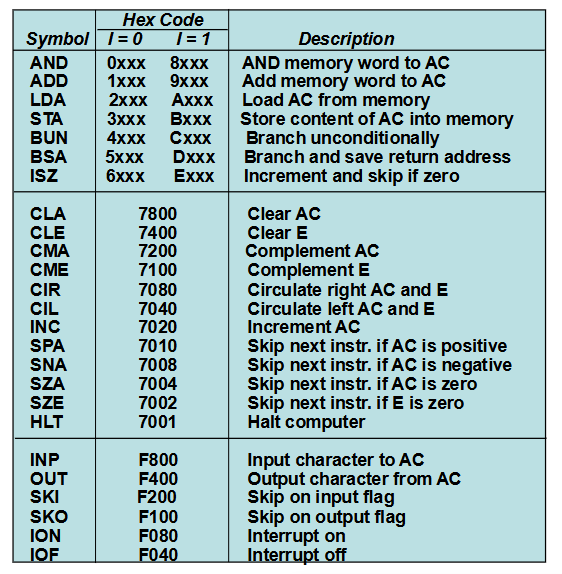
\includegraphics[width=0.5\textwidth]{10.1.png}
\end{center}

\subsection{Instruction Set Completeness}
\begin{itemize}
  \item If the computer includes a sufficent number of instructions in each category, it is considered a complete set of instructions.
  \begin{itemize}
    \item Arithmetic, logical and shift instructions
    \item Instructions for transfer interface between memory and CPU registers
    \item Input \& Output instructions
  \end{itemize}
\end{itemize}

\subsection{Timing Control}
\begin{itemize}
  \item Timing for all registers is controlled by a master clock generator
  \item Clock pulses are applied to \textbf{ALL} FFs and registers.
  \item Clock pulses \textbf{DO NOT} change states of a register \textbf{UNLESS} register is enabled by a control signal (ie Load)
  \item Control signals are generated by the control unit to control where data goes and what to do with it.
  \item Two types of control organization:
  \begin{itemize}
    \item Hardwired control
    \item Microprogrammed control
  \end{itemize}
\end{itemize}

\section{CPU Control Unit (CU)}
\begin{itemize}
  \item The control unit is a programmable sequential circuit whose transition $\delta$ and output $\lambda$ change relative to current instruction $I_14$ - $I_0$
  \item In a hardwired organization, CU consists of:
  \begin{itemize}
    \item 2 Decoders
    \item 1 Sequence Counter (SC)
    \item $N$ Control logic gates
  \end{itemize}
  \subitem Outputs from SC provide timing signals to $T_0$ to $T_15$
\end{itemize}
\subsection{Control Unit for the Basic Computer}
\begin{center}
  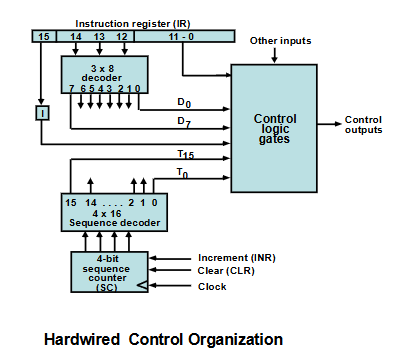
\includegraphics[width=0.7\textwidth]{10.2.png}
\end{center}
\begin{NumberedList}
  \item $IR_{15,12}$ is used for \textbf{data addressing} which is decoded by the 3x8 Decoder $D_{0,..,7}$.
  \item SC outputs timing signals $T_0$ to $T_15$ based on time, $t$. Each $T_n$ denotes a micro-operation (at most 1 clock pulse per $T_n$)
\end{NumberedList}
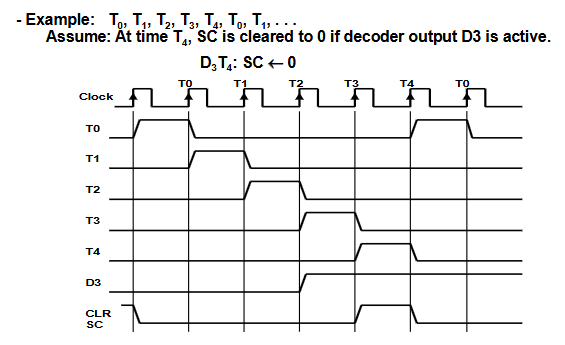
\includegraphics[width=1\textwidth]{10.3.png}
\section{Instruction Cycle}
\begin{itemize}
  \item Instructions are broken down into sub-cycles and phases
  \item Fetch and Decode
  \begin{itemize}
    \item $T_0$: AR $\leftarrow$ PC 
    \subitem Adress of the instruction is moved to AR
    \item $T_1$: IR $\leftarrow$ M[AR], PC $\leftarrow$ PC + 1
    \subitem Instruction is fetched from the memory to IR, PC is incremented 
    \item $T_2$: $D_0$ ,..., $D_7$ $\leftarrow$ IR(12-14), AR $\leftarrow$ IR(0-11), I $\leftarrow$ IR(15)
    \subitem Decodes $IR_{12-14}$ (which is the data addressing in the instruction code)
  \end{itemize}
  \begin{center}
    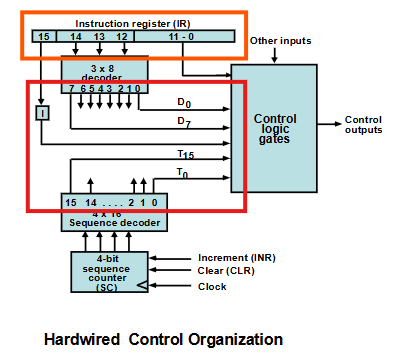
\includegraphics[width=0.6\textwidth]{10.4.png}
  \end{center}
  \begin{NumberedList}
    \item $T_0$ and $T_1$ are the fetch process (Orange)
    \item $T_2$ is the decoding process (Red)
  \end{NumberedList}
\end{itemize}



\end{document}
